\documentclass{amsart}
\usepackage{color}
\usepackage{amssymb, amsmath}
\usepackage{tikz}
\usepackage{tikz-cd}
\usetikzlibrary{snakes}
\usetikzlibrary{intersections, calc}

\begin{document}

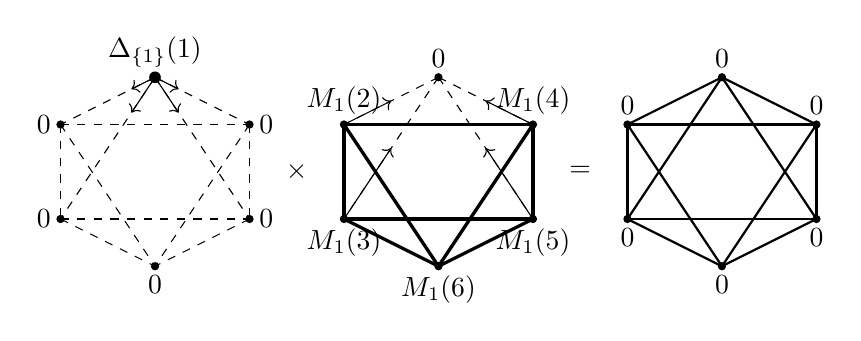
\begin{tikzpicture}
\begin{scope}[xscale=0.3, yscale=0.3]
\fill(0,4) circle (7pt);
\node[above] at (0,4) {$\Delta_{\{1\}}(1)$}; 
\fill(-4,2) circle (5pt);
\node[left] at (-4,2) {$0$};
\fill(-4,-2) circle (5pt);
\node[left] at (-4,-2) {$0$};
\fill(0,-4) circle (5pt);
\node[below] at (0,-4) {$0$};
\fill(4,-2) circle (5pt);
\node[right] at (4,-2) {$0$};
\fill(4,2) circle (5pt);
\node[right] at (4,2) {$0$};

\draw[dashed] (0,4)--(-4,2);
\draw[dashed] (0,4)--(-4,-2);
\draw[dashed] (0,4)--(4,-2);
\draw[dashed] (0,4)--(4,2);
\draw[dashed] (-4,2)--(-4,-2);
\draw[dashed] (-4,2)--(0,-4);
\draw[dashed] (-4,2)--(4,2);
\draw[dashed] (-4,-2)--(4,-2);
\draw[dashed] (-4,-2)--(0,-4);
\draw[dashed] (4,2)--(4,-2);
\draw[dashed] (4,2)--(0,-4);
\draw[dashed] (4,-2)--(0,-4);

\draw[->] (0,4)--(1,3.5);
\draw[->] (0,4)--(1,2.5);
\draw[->] (0,4)--(-1,2.5);
\draw[->] (0,4)--(-1,3.5);

\node at (6,0) {$\times$};

\fill(12,4) circle (5pt);
\node[above] at (12,4) {$0$};
\fill(8,2) circle (5pt);
\node[above] at (8,2) {$M_{1}(2)$};
\fill(8,-2) circle (5pt);
\node[below] at (8,-2) {$M_{1}(3)$};
\fill(12,-4) circle (5pt);
\node[below] at (12,-4) {$M_{1}(6)$};
\fill(16,-2) circle (5pt);
\node[below] at (16,-2) {$M_{1}(5)$};
\fill(16,2) circle (5pt);
\node[above] at (16,2) {$M_{1}(4)$};

\draw[dashed] (12,4)--(8,2);
\draw[dashed] (12,4)--(8,-2);
\draw[dashed] (12,4)--(16,-2);
\draw[dashed] (12,4)--(16,2);
\draw[very thick] (8,2)--(8,-2);
\draw[very thick] (8,2)--(12,-4);
\draw[very thick] (8,2)--(16,2);
\draw[very thick] (8,-2)--(16,-2);
\draw[very thick] (8,-2)--(12,-4);
\draw[very thick] (16,2)--(16,-2);
\draw[very thick] (16,2)--(12,-4);
\draw[very thick] (16,-2)--(12,-4);

\draw[->] (8,2)--(10,3);
\draw[->] (8,-2)--(10,1);
\draw[->] (16,-2)--(14,1);
\draw[->] (16,2)--(14,3);

\node at (18,0) {$=$};

\fill(24,4) circle (5pt);
\node[above] at (24,4) {$0$};
\fill(20,2) circle (5pt);
\node[above] at (20,2) {$0$};
\fill(20,-2) circle (5pt);
\node[below] at (20,-2) {$0$};
\fill(24,-4) circle (5pt);
\node[below] at (24,-4) {$0$};
\fill(28,-2) circle (5pt);
\node[below] at (28,-2) {$0$};
\fill(28,2) circle (5pt);
\node[above] at (28,2) {$0$};

\draw[thick] (24,4)--(20,2);
\draw[thick] (24,4)--(20,-2);
\draw[thick] (24,4)--(28,-2);
\draw[thick] (24,4)--(28,2);
\draw[thick] (20,2)--(20,-2);
\draw[thick] (20,2)--(24,-4);
\draw[thick] (20,2)--(28,2);
\draw[thick] (20,-2)--(28,-2);
\draw[thick] (20,-2)--(24,-4);
\draw[thick] (28,2)--(28,-2);
\draw[thick] (28,2)--(24,-4);
\draw[thick] (28,-2)--(24,-4);
\end{scope}
\end{tikzpicture}

\end{document}